\pdfminorversion=4
\documentclass{beamer}

\usetheme{Madrid}

\usepackage[ngerman]{babel}
\usepackage[T1]{fontenc}
\usepackage[utf8]{inputenc}
\usepackage{graphicx}
\usepackage{hyperref}
\usepackage{tikz}
\usepackage{color}
\usepackage{epsfig}
\usepackage{bytefield}

\makeatletter
\newcommand{\rmnum}[1]{\romannumeral #1}
\newcommand{\Rmnum}[1]{\expandafter\@slowromancap\romannumeral #1@}
\makeatother

\title{Das Vaporschloss}
\author{florolf}
\institute{Entropia}
\date{6. November 2011}

\begin{document}
\begin{frame}
  \titlepage
\end{frame}

\begin{frame}{Anforderungen}
  \begin{itemize}
  \item Schl\"usseldiffusion reduzieren
    \begin{itemize}
    \item Kopieren verhindern
    \item Einzelne Schl\"ussel revoken
    \end{itemize}
  \item Fallback auf Hardwareschl\"ussel
  \item Trackbarkeit verhindern
  \end{itemize}
\end{frame}

\begin{frame}{Vaporschloss Mk \Rmnum{1}}
  \begin{itemize}
  \item 125 kHz RFID
  \item Trivial Klonbar
  \item Wackelige Pollin-Konstruktion
  \item Nicht fertiggeworden
  \end{itemize}
\end{frame}

\begin{frame}{Vaporschloss Mk \Rmnum{2}}
  \begin{itemize}
  \item Mifare DESFire EV1
    \item Intelligentes RFID auf 13,56 MHz
      $\Rightarrow$
      \begin{itemize}
      \item (hoffentlich) nicht klonbar
      \item flexibler
      \item Aber: Trackbar
    \end{itemize}
  \item Fertig? (Neingeist glaubt's erst, wenn er damit die T\"ur
    aufgemacht hat)
  \end{itemize}
\end{frame}

\begin{frame}{Mifare DESFire}{Sie haben gelernt}
  \begin{itemize}
  \item ISO 14443-4-Kompatibel
  \item Gegenseitige Authentifikation (Reader $\leftrightarrow$ Karte)
  \item 2.5DES
  \item AES (Nur unter NDA)
    \pause
  \item Naja, fast:
    \begin{itemize}
    \item Differential Power Analysis-Attacke gegen DESFire vor EV1
      \begin{itemize}
      \item EV1 ist EAL4+ {\textbackslash}o/
      \end{itemize}
    \item Stellenweise theoretisch Replay-Attacken m\"oglich
    \end{itemize}
  \end{itemize}
\end{frame}

\begin{frame}{Was geht?}
  \begin{block}{Platz}
    \begin{itemize}
    \item 1, \textbf{2}, \textbf{4}, 8 kB Speicher
    \item Bis zu 28 Anwendungen
    \item Bis zu 14 Schl\"ussel pro Anwendung
    \item Bis zu 16 Dateien pro Anwendung
    \end{itemize}
  \end{block}
  \pause
  \begin{block}{Dateitypen}
    \begin{itemize}
    \item (Backup) Data files
    \item Value files
    \item Linear/Cyclic record files
    \end{itemize}
  \end{block}
  \pause
  \begin{block}{Policy}
    \begin{itemize}
    \item Eindeutige UID
    \item Berechtigungen auf Karte/Anwendungen/Dateien
    \end{itemize}
  \end{block}
\end{frame}

\begin{frame}{Schl\"ussel und Berechtigungen}
  \begin{block}{AID 0}
    \begin{itemize}
    \item "`Die Karte"'
    \item Keine Dateien
    \item Nur ein Schl\"ussel: PICC Master Key
    \item Karte l\"oschen, Applikationen erstellen/l\"oschen,
      Einstellungen \"andern, Karte einfrieren
    \end{itemize}
  \end{block}
  \begin{block}{Rest}
    \begin{itemize}
    \item Bis zu 14 Schl\"ussel
    \item Schl\"usselid 0: Application Master Key (AMK)
    \item Beliebige Kombinationen von Berechtigungen auf Schl\"ussel
    \end{itemize}
  \end{block}
\end{frame}

\begin{frame}[fragile]{Dateiberechtigungen}
  \begin{center}
    \begin{bytefield}[bitwidth=1.7em]{16}
      \bitheader{0-15} \\
      \bitbox{4}{Change Access} & \bitbox{4}{Read \& Write} &
      \bitbox{4}{Write} & \bitbox{4}{Read}
    \end{bytefield}
  \end{center}

  \begin{block}{Magische Schl\"ussel}
    \begin{description}
    \item[\texttt{E}] Jeder
    \item[\texttt{F}] Keiner
    \end{description}
  \end{block}
\pause
  \begin{block}{Value files}
    \begin{description}
      \item[Read] GetValue, Debit
      \item[Write] LimitedCredit + \textcolor{beamer@blendedblue}{Read} 
      \item[Read\&Write] Credit + \textcolor{beamer@blendedblue}{Write} 
    \end{description}
  \end{block}
\end{frame}

\begin{frame}{Kommunikationsmodus}
  \begin{block}{Modi}
    \begin{description}
    \item[\texttt{0}] Plain
    \item[\texttt{1}] MACed
    \item[\texttt{3}] Crypted
    \end{description}
  \end{block}
\pause
  \begin{alertblock}{Achtung}
    Wenn eine relevante Zugriffsberechtigung \texttt{E} ist
    $\Rightarrow$ Plain
  \end{alertblock}
\pause
\begin{block}{Crypted}
  \begin{itemize}
  \item CRC16 anh\"angen, DES mit CBC
  \item IV immer \texttt{0000000000000000}
  \end{itemize}
\end{block}
\end{frame}

\begin{frame}{Authentifikation}
  \begin{center}
    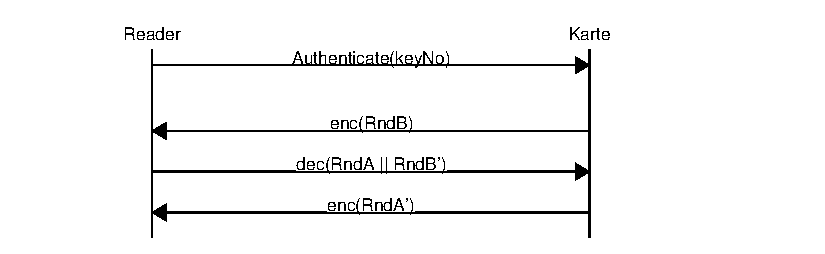
\includegraphics{auth.eps} \\
    $RndX' = rol(RndX, 8)$\\
    $sk = RndA1 || RndB1 || RndA2 || RndB2$
  \end{center}
\end{frame}

\begin{frame}{Hardware}
  \begin{center}
    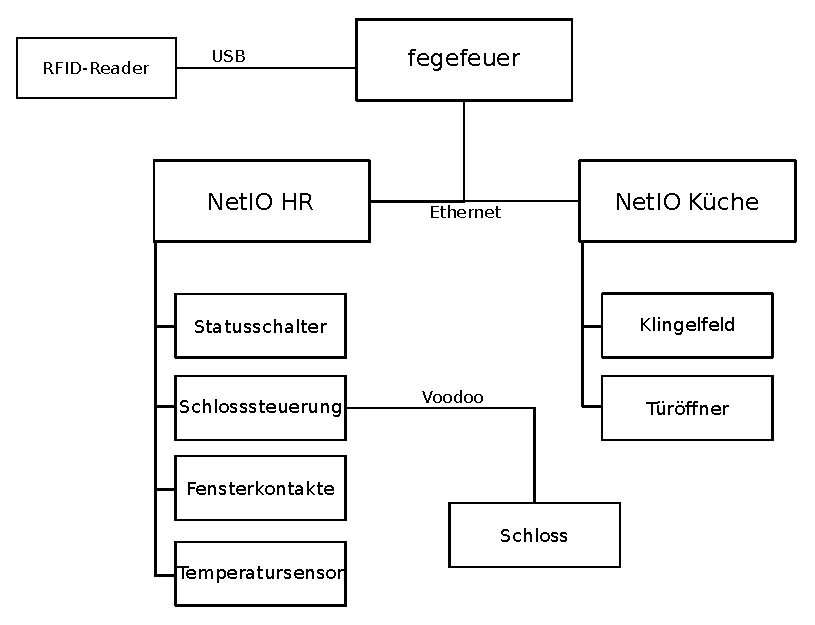
\includegraphics[height=.7\textheight]{hardware.eps}
  \end{center}
\end{frame}

\begin{frame}{Software}
  \begin{center}
    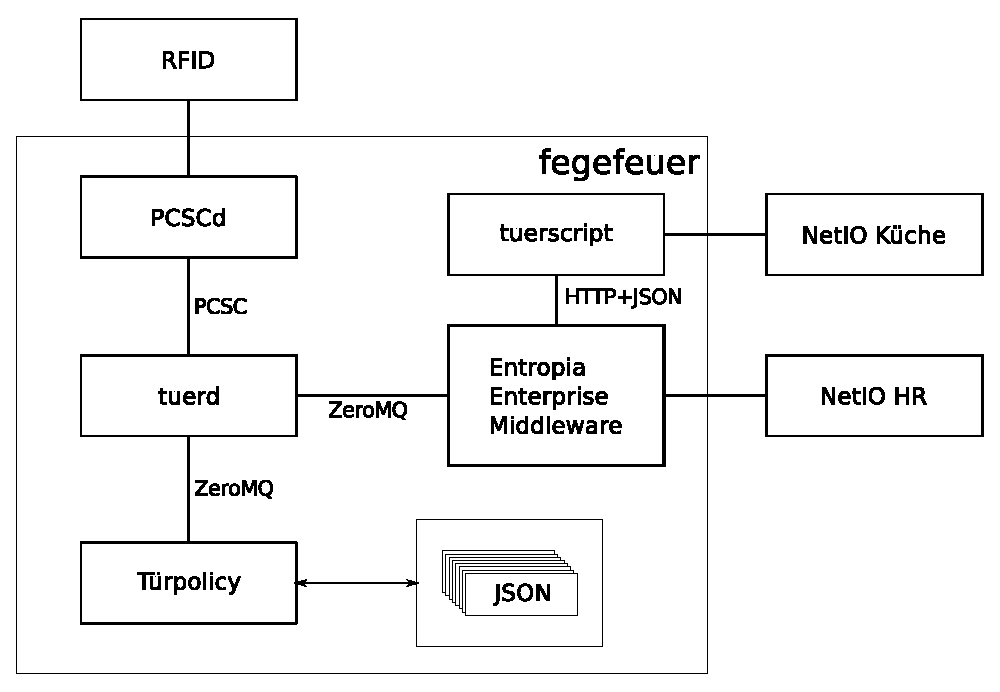
\includegraphics[height=.7\textheight]{software.eps}
  \end{center}
\end{frame}

\begin{frame}[fragile]{JSON}
  \begin{center}
    \begin{verbatim}
{
    "user": "florolf",
    "buergen": ["foo", "bar", "qux"],
    "card": {
        "uid": "00010203040506",
        "picc_key": "6997FA088A3E9079B609B85CC81844C5",
        "ca0523_amk": "13F64D4F452FEBB56010F8A981CC82FB",
        "ca0523_door_key": "D7001CF78B91CBEF6350EB25832E17F3"
    }
}
    \end{verbatim}
  \end{center}
\end{frame}

\begin{frame}{T\"ur}
  \begin{block}{Daten auf der Karte}
    \begin{itemize}
    \item Applikation: \texttt{0xCA0523}
    \item Schl\"ussel \texttt{0xD} (shared secret mit der T\"ur)
    \end{itemize}
  \end{block}
  \begin{enumerate}
  \item \emph{GetVersion}() $\rightarrow$ UID
  \item Schl\"ussel nachschlagen
  \item \emph{SelectApplication}(\texttt{0xCAO523})
  \item \emph{Authenticate}(\texttt{0xD})
  \end{enumerate}
\end{frame}

\begin{frame}{Und weiter?}
  \begin{itemize}
  \item Getr\"ankekasse
  \item Bessere Kryptographie (z.B. kontaktlose JavaCards)
  \item Selber rumspielen
  \end{itemize}
\end{frame}

\begin{frame}
  \begin{center}
    \Huge Fragen?
  \end{center}
\end{frame}

\end{document}
